\section{Lecture 25: Interior Point Method}
In last lecture, we have discussed about Newton's method. One advantage is its fast local convergence rate. However, there is no guarantee on global convergence for Newton's method. In this lecture, we'll present interior point method, which can be considered as an extension of Newton's method to ensure global convergence. First, the idea of interior point method will be introduced for general constrained optimization problems. Then the detailed algorithm and its convergence will be explained for linear programming. 
\subsection{Barrier Methods}
We'll firstly introduce barrier methods which convert the inequality constraints into a function added upon the objective function of a optimization problem. Consider the following optimization problem: 
\begin{equation}
\begin{aligned}
&\min_x & {f(x)}\\
&\qquad\text{s.t.} &x&\in{\domain},\\
& &g_j(x)&\leqslant{0},\ j=1,2,\cdots,r,\\
\end{aligned}
\end{equation}
where $f:\R^n\rightarrow\R$, $g_j:\R^n\rightarrow\R$ are given functions. $f$ is continuous, and $\domain$ is a closed set. For the rest of the lecture, we assume convex $g_j$ and $\domain=\R^n$. And we denote $x^*$ as the optimal solution of the problem.

\begin{definition}[Interior of the constraint region]
The interior (relative to $\domain$) of the constraint region is defined as $S=\{x\in\domain:g_j(x)<0,\ j=1,2,\cdots,r\}$. 

Assuming nonempty and convex $S$, we define a so-called barrier function $B(x)$ defined on $S$, such that $B(x)$ is continuous and $\lim_{g_j(x)\rightarrow{0_{\_}}}B(x)=\infty$. Two most common examples are logarithmic barrier function and inverse barrier function: 
\begin{align}
\text{Logarithmic:}\qquad B(x) &= -\sum_{j=1}^{r}\ln\{-g_j(x)\}\\
\text{inverse:}\qquad B(x) &= -\sum_{j=1}^{r}\frac{1}{g_j(x)}.
\end{align}
Both of them are convex if all $g_j(x)$ are convex. 

\begin{figure}[ht]
\centering
\includegraphics[scale=0.4]{figures/lecture25-barrier_function}
\caption{Form of a barrier term}
\label{fig:barrier}
\end{figure}

Given $B(x)$, define a new cost function $f_\epsilon(x)=f(x)+\epsilon{B(x)}$, where $\epsilon$ is a positive real number. Then we can eliminate the inequality constraints in the original problem and obtain the following problem: 
\begin{equation}
\begin{aligned}
&\min_x & {f_\epsilon(x)}\\
&\qquad\text{s.t.} & x\in{\domain},\\
\end{aligned}
\end{equation}
The form of the barrier term $\epsilon{B(x)}$ is illustrated in Figure \ref{fig:barrier}.

The barrier method is defined by introducing a sequence $\{\epsilon_t\}$ such that $0<\epsilon_{t+1}<\epsilon_t$ for $t=0,1,2,...$ and $\epsilon_t\rightarrow{0}$. Then we find a sequence $\{x_t\}$ such that $x_t\in{\arg \min_{x\in{S}}}f_{\epsilon_t}(x)$. Note that the barrier term $\epsilon_t{B(x)}$ goes to zero for all interior points $x\in{S}$ as $\epsilon_t\rightarrow{0}$, allowing $x_t$ to get increasingly closer to the boundary. Therefore, intuitively, $x_t$ should approach $x^*$ no matter $x^*$ is in the interior or on the boundary of $S$. Its convergence is formalized in the following proposition. 

\begin{proposition}
Every limit point of a sequence $\{x_t\}$ generated by a barrier method is a global minimum of the original constrained problem. 
\end{proposition}
\begin{proof}
See Proposition 5.1.1 of \cite{bertsekas2016nonlinear}.
\end{proof}

As $\domain=\R^n$, Newton's method can be applied with properly selected stepsize to ensure that all iterates lies in $S$. Concretely, an initial interior point can be obtained for some large $\epsilon_0$. Then in each iteration, we can use $x_t$ as an initialization to find $x_{t+1}$ by Newton's method. When $\epsilon_0$ is large, it is easier to find a interior point. And since $x_t$ is close to $x_{t+1}$, it is likely that $x_t$ is in the local convergence region for Newton's method. Therefore, intuitively, global convergence of Newton's method can be enabled by using barrier methods.


\end{definition}
\subsection{Linear Programming}
We'll now adopt the logarithmic barrier method to solve the linear programming (LP) problem defined as follows:
\begin{equation}
\label{eq:LP_def}
\text{LP}:\qquad
\begin{aligned}[c|c|c]
&\min_x &c^T&x\\
&\qquad\text{s.t.} &Ax&\ge b
\end{aligned}
\end{equation}
where $A\in\mathbb{R}^{m\times n}$ with $m\ge n$ and rank($A$)=n. Denote $x^*$ as the optimal point. 

First we write out the augmented cost function by the logarithmic barrier method, i.e.,
\begin{equation}
\label{eq:LP_aug_cost}
f_\epsilon(x) = c^T x-\epsilon \sum_{j=1}^m\ln\left(A^T_j x-b\right).
\end{equation}
where $A^T_j$ is the $j$-th row of $A$. Define $x^*_\epsilon=\argmin_x f_\epsilon(x)$. 

\noindent\textbf{Fact}: $x^*_\epsilon$ exists and is unique for any $\epsilon>0$.
\begin{proof}
We can easily check that $f_\epsilon(x)$ is convex (as a sum of two convex functions). Therefore, the minimizer $x^*_\epsilon$ must exist and is unique.

\textit{Remark}: For the convexity of $f_\epsilon$, we can also check the second-order derivative, which is positive definite as shown in (\ref{eq:hessian_f_eps}) later.
\end{proof}

\subsubsection{Central Path}
The central path of the LP problem in \ref{eq:LP_def} is depicted by the set of $\left\{x^*_\epsilon|\epsilon>0\right\}$, as shown in Fig.~\ref{fig:central_path}.
\begin{figure}[h!]
\centering
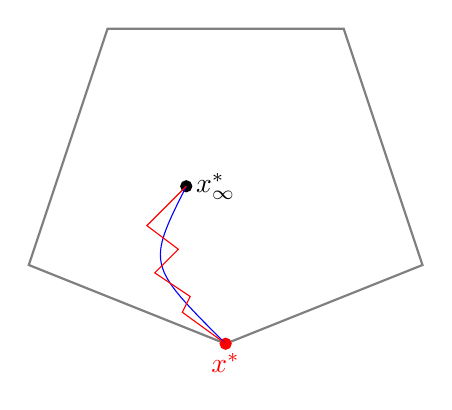
\begin{tikzpicture}
\draw[gray, thick] (-1,2) -- (2,2) -- (3,-1) -- (0.5,-2) -- (-2,-1) -- cycle;
\filldraw[black] (0,0) circle (2pt) node[anchor=west] {$x^*_\infty$};
\filldraw[red] (0.5,-2) circle (2pt) node[anchor=north] {$x^*$};
\draw[blue, thin] (0,0) .. controls (-0.5,-1) .. (0.5,-2);
\draw[red, thin] (0,0) -- (-0.5,-0.5) -- (-0.1,-0.8) -- (-0.4,-1.1) -- (0.05,-1.4) -- (-0.05,-1.6) -- (0.5,-2);
\end{tikzpicture}
\caption{The central path\label{fig:central_path}}
\end{figure}

Our goal is to design an algorithm that will approximately follow the central path. Assume that we already get a "good" enough initial point, then at every step, we apply one step of Newton's method. To guarantee that the algorithm converges, we need to answer the following two questions:
\begin{itemize}
\item Under what conditions that the single-step Newton method works?
\item How to carefully update $\epsilon$?
\end{itemize}

\subsubsection{Newton Decrement}
To apply the Newton's method, first we need to find out the first-order and second-order derivatives of $f_\epsilon$. Note that
\begin{eqnarray}
\triangledown f_\epsilon(x)&=&c-\epsilon \sum_{j=1}^m \dfrac{A_j}{A^T_j x-b}\triangleq c-\epsilon A^T S^{-1}\mathbb{1}\label{eq:grad_f_eps}\\
\triangledown^2f_\epsilon(x)&=&\epsilon A^TS^{-2}A=\epsilon \sum_{j=1}^m\dfrac{A_j A_j^T}{S_j^2}\label{eq:hessian_f_eps}
\end{eqnarray}
where $\mathbb{1}=[1,1,\cdots,1]^T\in\mathbb{R}^{m\times1}$, $S=diag\{A^T_1 x-b, A^T_2 x-b, \cdots, A^T_m x-b\}$.

Then the Newton's update can be applied:
\begin{equation}
\bar{x}=x-[\triangledown^2f_\epsilon(x)]^{-1}\triangledown f_\epsilon(x)=x-[\epsilon A^TS^{-2}A]^{-1}\left(c-\epsilon A^T S^{-1}\mathbb{1}\right)\label{eq:Newton_update}
\end{equation}

Recall that the Newton's method finds the solution by making the first-order condition zero. To measure how much the Newton update will decrease the first-order approximation, we introduce the concept of Newton decrement.

Define the Newton decrement as
\begin{equation}
q^2(x, \epsilon) = \triangledown f^T_\epsilon(x)[\triangledown^2f_\epsilon(x)]^{-1}\triangledown f_\epsilon(x)\label{eq:newton_decrement}
\end{equation}
or $q(x, \epsilon) = [\triangledown^2f_\epsilon(x)]^{-1/2}\triangledown f_\epsilon(x)$. 

Note that the Newton decrement also relates to the difference between $f_\epsilon(x)$ and the minimum of its second-order approximation:
\begin{eqnarray}
&&f_\epsilon(x)-\min_{\bar{x}}\left(f_\epsilon(x)+\triangledown f_\epsilon(x)^T(\bar{x}-x)+(\bar{x}-x)^T\triangledown^2 f_\epsilon(x)(\bar{x}-x)\right)\nonumber\\
&=&f_\epsilon(x)-\left(f_\epsilon(x)-\dfrac{1}{2}\triangledown f^T_\epsilon(x)[\triangledown^2f_\epsilon(x)]^{-1}\triangledown f_\epsilon(x)\right)\nonumber\\
&=&\dfrac{1}{2}\triangledown f^T_\epsilon(x)[\triangledown^2f_\epsilon(x)]^{-1}\triangledown f_\epsilon(x)\triangleq \dfrac{1}{2}q^2(x, \epsilon).
\end{eqnarray}

We now will use the Newton decrement to answer the above two questions: conditions for single-step Newton to work and rules for updating $\epsilon$.

\subsubsection{Propositions, Algorithms and Convergence Theorem}
\begin{proposition}\label{prop1}
Assume $Ax > b$ and $\|q(x, \epsilon)\|<1$, then we have
\begin{align}
c^Tx-c^Tx^{*}\leq 2\epsilon n.
\end{align}
\end{proposition}
In particular, if we maintain that $x_t$ is interior point satisfying $Ax_t>b$,
and $q(x_t, \epsilon_t) < 1$, then $c^{T}x_t$ converges to $c^Tx^*$ as $\epsilon_t$ goes to $0$, i.e., $x_t$ converges to global optimum. However, the condition $q(x_t,\epsilon_t)<1$ is not trivial.  

\begin{proposition}\label{prop2}
If $Ax>b$, and $q(x,\epsilon)<1$, then the pure Newton iterate
step $\bar{x}$ satisfies,
\begin{align}
\|q(\bar{x}, \epsilon)\| &\leq \|q(x, \epsilon)\|^2 
\end{align}
\end{proposition}
It ensures that $\|q(\bar{x}, {\epsilon})\|<1$ given $q(x,\epsilon)<1$ and $x$ is interior point. But we also want that $\|q(\bar{x}, \bar{\epsilon})\|<1$ for some $\bar{\epsilon}<\epsilon$. 

\begin{proposition}\label{prop3}
Assume $q(x,\epsilon)\leq \frac{1}{2}$, interior point $Ax>b$,
put 
\begin{align}
\bar{\epsilon} = (1-\frac{1}{6\sqrt{n}})\epsilon,
\end{align}
then we have
\begin{align}
\|q(\bar{x}, \bar{\epsilon})\|\leq \frac{1}{2}
\end{align}
\end{proposition}
These propositions indicates the following update rule,
\begin{align}
x_{t+1} & = x_t - \nabla^Tf_{\epsilon_t}(x)^{-1}\nabla f_{\epsilon_t}(x_t) \\
\epsilon_t & = (1-\frac{1}{6\sqrt{n}})\epsilon
\end{align}
\begin{theorem}
Suppose $(x_0, \epsilon_0)$ satisfies $Ax_0 >b$ and 
$\|q(x_0,\epsilon_0)\|\leq\frac{1}{2}$, then the algorithm
converges in $\mathcal{O}(\sqrt{n}\log(n/\eta))$ iterations to $\eta$ error, i.e., we have $c^Tx_t\leqslant{c^Tx^*+\eta}$ after $\mathcal{O}(\sqrt{n}\log(n/\eta))$ iterations.
\end{theorem}

\begin{proof}
As Newton step maintains $x_{t+1}$ in the interior, by using the three propositions above, we have 
\begin{eqnarray}
c^Tx_t&\leqslant&{c^Tx^*+2\epsilon_t{n}}\nonumber\\
&=&{c^Tx^*+2(1-\frac{1}{6\sqrt{n}})^t\epsilon_0}\nonumber\\
&\leqslant&{c^Tx^*+2\exp(-\frac{t}{6\sqrt{n}})\epsilon_0}
\end{eqnarray}
Therefore, to have a error of $\eta$, $t\geqslant{\frac{6\sqrt{n}}{\epsilon_0}}\log{\frac{2n}{\eta}}$. We can then conclude that the algorithm converges in  $\mathcal{O}(\sqrt{n}\log(n/\eta))$ iterations to $\eta$ error. 
\end{proof}

The algorithm stated above is the so-called short-step method. Although theoretical convergence rate is guaranteed, the combination of small decrease in $\epsilon$ and a single Newton step is slow in practice. Instead, a more practical method is the so-called long-step method, where $\epsilon$ is reduced in faster rate and several Newton steps are taken per iteration.
